\documentclass[12pt]{article}
  \usepackage[francais]{babel}
  \AddThinSpaceBeforeFootnotes % à insérer si on utilise \usepackage[french]{babel}
  \FrenchFootnotes % à insérer si on utilise \usepackage[french]{babel}
  \usepackage[T1]{fontenc}
  \usepackage[utf8]{inputenc}
  \usepackage{graphicx}
  \usepackage[left=2.5cm,right=2.5cm,top=2.5cm,bottom=2.5cm]{geometry}
  \usepackage{array}
  \usepackage{booktabs}
  \usepackage[squaren,Gray]{SIunits}  % Unité ex: $\unit{5 \cdot 10^{-6}}{\meter}$
  \usepackage{colortbl}               % Pour les couleur des cellules (tableau)
  \usepackage{amsmath}				  % Pour les formules mathématiques
  \usepackage{upgreek}                % Pour les lettres greque
  %\usepackage{fullpage}	          % plus petites marges
  \usepackage{verbatim}				  % Pour de long commentaires
  \usepackage[lofdepth,lotdepth]{subfig}       % Faire des sous-figures
  \usepackage{url}
  \usepackage{colortbl}               % pour les couleur des cellules (tableau)
  \usepackage{indentfirst}
  \usepackage{multirow}
  \usepackage{xfrac}
  \usepackage{wrapfig}
  \usepackage{enumitem}               % Liste personnalisée
  \frenchbsetup{StandardLists=true}   % Empêche conflits entre enumitem et babel
  \usepackage{placeins}   % place une barrière pour que l'image/table soit derrière \FloatBarrier
  \usepackage{lastpage} 
  \usepackage{titling}
  \usepackage{lmodern}
  \usepackage{booktabs}
  \usepackage{etoolbox}
  \usepackage[most]{tcolorbox}
  
  
  %Change la taille de police
  \newcommand\ChangeRT[1]{\noalign{\hrule height #1}}
  
\graphicspath{{images/}}

  
  %Création  d'une nouvelle commande pour faire référence à une Figure
  %Exemple : \appelFigure{schema} donne : Figure 1 (en italique)
  \newcommand{\appelFigure}[1]{
    \textit{Figure \ref{#1}}
  }
      
  %%Création commande pour insérer image avec nom de figure directement
  %\newcommand{nomDeTaCommande}[nombreArguments]{CodeLaTeX}
  %\insertImage[position]{image_path}{scale}{Titre_figure}{label}
  \newcommand{\insertImage}[5][center]{
      \begin{#1}
      \includegraphics[scale=#3]{#2}
      \captionof{figure}{#4} 
      \label{#5}
      \end{#1}
  }

  % Affichage des frames pour commande cisco
  \newtcblisting{cisco}[1][]{size=fbox, listing only, listing options={style=tcblatex,basicstyle=\ttfamily\scriptsize,tabsize=2,language=sh},title=#1}

  %En-tête et pied de page personalisé
  \usepackage{fancyhdr}
  \pagestyle{fancy}
  \fancyhf{}
  \setlength\parindent{0pt} %Supprime les alinéa
  \setlength{\parskip}{8pt} %Augmente l'espace entre paragraphe
  %Bottom numbering page
  \renewcommand{\headrulewidth}{1pt}
  \fancyhead[L]{
\includegraphics[scale=.2]{heia-fr-logo.png}}
  \fancyhead[R]{\theauthor}
  
  \renewcommand{\footrulewidth}{1pt}
  \fancyfoot[R]{\textbf{Page \thepage\ sur \pageref{LastPage}}} 
%  \fancyfoot[L]{\leftmark}

  \setlength\parindent{0pt} %Supprime les alinéa
  \setlength{\parskip}{8pt} %Augmente l'espace entre paragraphe

 
\title{Résumé OS de mort} 
\author{\textsl{Marc} \textsc{Roten}}
\date{}

 
 
\begin{document}
    \begin{titlepage}
        \begin{center}
            
\includegraphics[scale=.4]{Img/heia-fr-logo.png}\\[1.3cm]
            
            \rule{\linewidth}{0.3mm} \\[0.3cm]
            {\huge \bfseries Operating Systems\\[0.5cm]} 
            {\Large  Résumé TE02 }
            \rule{\linewidth}{0.3mm} \\[0.8cm]
            \noindent{}
            \begin{minipage}[t]{0.4\textwidth} 
                \begin{flushleft} \large
                    \emph{Auteur :}\\
                    \theauthor
                \end{flushleft}
            \end{minipage}
            \begin{minipage}[t]{0.4\textwidth} 
                \begin{flushright} \large
                    \emph{Professeur:}\\
                    \textsl{Jacques} \textsc{ Supcik}\\ 
                \end{flushright} 
                \vfill
            \end{minipage}\\[1.3cm]
            
\includegraphics[scale=0.3]{Img/title.jpg}\\[1.5cm]
            \vspace*{1\baselineskip}
            \today \\[0.7cm]
        \end{center}
    \end{titlepage}
    \tableofcontents
    \clearpage 
% \insertImage{Img/photo.PNG}{0.8}{Schéma explicatif}{}

% \section{voici comment faire un chapitre}
 
%     \subsection{Voici comment faire un sous chapitre}

% \section{des commandes}
%     \subsection{commande cisco}
    
%     \begin{cisco}[une commande sympa type cisco]
%       un texte lambda
%     \end{cisco}
    
%     \subsection{commande cisco allégée}
    
%     \begin{cisco}
%       un texte lambda
%     \end{cisco}
    
    
%     \subsection{commande pour mettre une image}
    
%     % \insertImage{Img/1.PNG}{echelle pour l'image (source = 1)}{texte dessous l'image}{référence vers l'objet
%     \insertImage{Img/1.JPG}{0.6}{voici une image}{}
%       \insertImage{Img/27.JPG}{0.6}{}{}

\section{Introduction}
Résumé pour la deuxième inter d'OS. Spécial dédicace à ma mère, pour la fête des mères.\\[5.5cm]
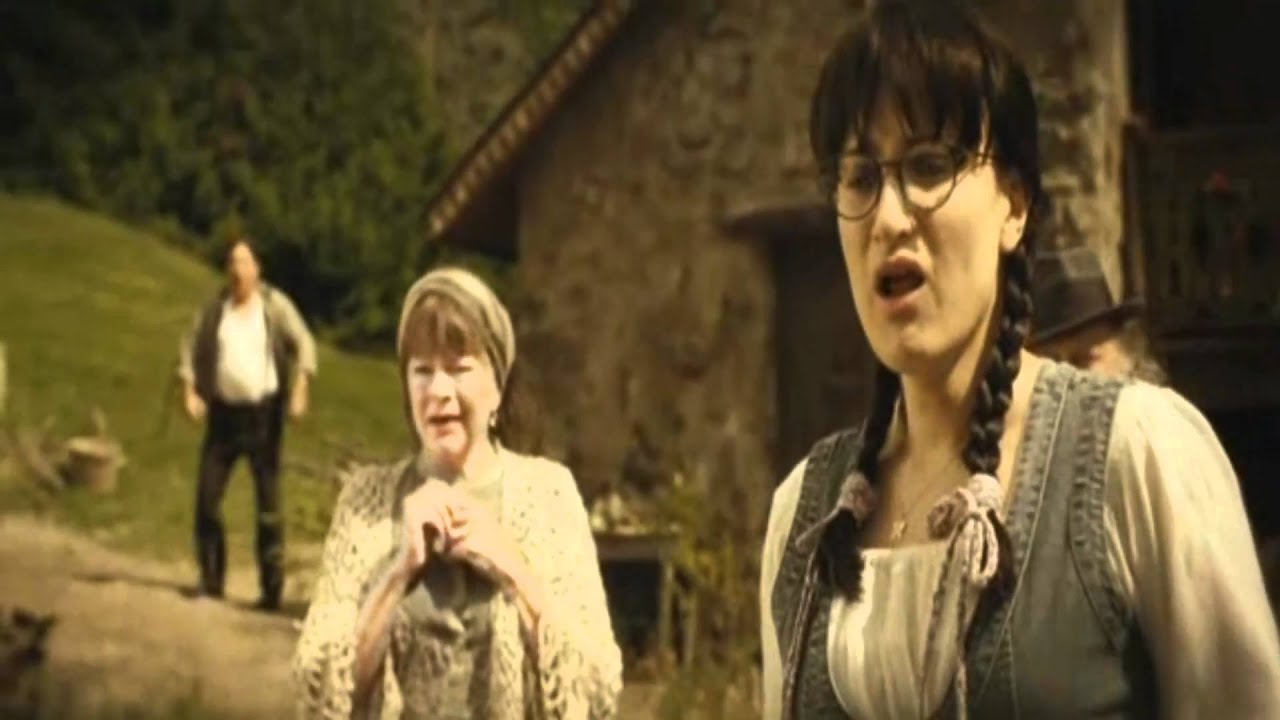
\includegraphics[scale=.35]{Img/0.PNG}
\newpage
\section{Chapitre\_6 La Gestion de la Mémoire}
\subsection{TLB toussa toussa}
TODO
\subsection{Page Replacement Algorythm}
TODO
\newpage
\section{Chapitre\_7 Systèmes de fichiers}%DONE
\insertImage{Img/1.PNG}{0.6}{Problèmes avec la RAM}{}

All computer applications need to store and retrieve information. While a process is running, it can store a limited amount of information within its own address space. However, the storage capacity is restricted to the size of the virtual address space. For some applications this size is adequate, but for others, such as airline reservations, banking, or corporate record keeping, it is far too small. A second problem with keeping information within a process’ address space is that when the process terminates, the information is lost. For many applications (e.g., for databases), the information must be retained for weeks, months, or even forever. Having it vanish when the process using it terminates is unacceptable. Furthermore, it must not go away when a computer crash kills the process. A third problem is that it is frequently necessary for multiple processes to access (parts of) the information at the same time. If we have an online telephone directory stored inside the address space of a single process, only that process can access it. The way to solve this problem is to make the information itself independent of any one process. Thus, we have three essential requirements for long-term information storage:
\begin{itemize}
    \item It must be possible to store a very large amount of information.
    \item The information must survive the termination of the process using it.
    \item Multiple processes must be able to access the information at once.
\end{itemize}
for the moment, it is sufficient to think of a disk as a linear sequence of fixed-size blocks and supporting two operations:
\begin{itemize}
    \item Read Block k
    \item Write Block k
\end{itemize}

Questions who pops out at this point in this chapter: 
\begin{itemize}
    \item How do we find the information?
    \item How do we avoid user from reading others user's Data?
    \item How do we know if a block is free?
\end{itemize}

\subsection{New Abstraction: the File}
The system file used to take care of the files is names \textbf{File System}.A file is an abstraction mechanism. It provides a way to store information on the disk and read it back later. This must be done in such a way as to shield the user from the details of how and where the information is stored, and how the disks actually work.

Windows 95 and Windows 98 both used the MS-DOS file system, called FAT-16, and thus inherit many of its properties, such as how file names are constructed. Windows 98 introduced some extensions to FAT -16, leading to FAT-32, but these two are quite similar. In addition,Windows NT, Windows 2000, Windows XP, Windows Vista, Windows 7, and Windows 8 all still support both FAT file systems, which are really obsolete now.
\subsubsection{File Name}                                                

Many operating systems support two-part file names, with the two parts separated by a period, as in prog.c. The part following the period is called the file extension and usually indicates something about the file. In MS-DOS, for example, file names are 1 to 8 characters, plus an optional extension of 1 to 3 characters. In UNIX, the size of the extension, if any, is up to the user, and a file may ev en hav e two or more extensions, as in homepage.html.zip, where .html indicates a Web page in HTML and .zip indicates that the file (homepage.html) has been compressed using the zip program.


\subsubsection{File system Examples}                                                
\insertImage{Img/5.PNG}{0.6}{File systems examples}{}

\subsubsection{File extensions}
\insertImage{Img/4.PNG}{0.6}{Most common extensions}{}

\subsubsection{File Structure}
\insertImage{Img/struct.PNG}{0.6}{File structure}{stru}

The figure \ref{stru}a, is an unstructured sequence of bytes. In effect, the operating system does not know or care what is in the file. All it sees are bytes. Any meaning must be imposed by user-level programs. Both UNIX and Windows use this approach.

The figure \ref{stru}b, In this model, a file is a sequence of fixed-length records, each with some internal structure. Central to the idea of a file being a sequence of records is the idea that the read operation returns one record and the write operation overwrites or appends one record.

The figure \ref{stru}c, The third kind of file structure is shown in Fig. 4-2(c). In this organization, a file consists of a tree of records, not necessarily all the same length, each containing a key field in a fixed position in the record. The tree is sorted on the key field, to allow rapid searching for a particular key. The basic operation here is not to get the ‘‘next’’ record, although that is also possible, but to get the record with a specific key.

\subsubsection{File type}
\insertImage{Img/6.PNG}{0.6}{FileName}{}
\insertImage{Img/7.PNG}{0.6}{FileName}{}
\insertImage{Img/8.PNG}{0.6}{FileName}{}
\insertImage{Img/9.PNG}{0.6}{FileName}{}



\subsection{Ordinary file}
\subsubsection{Text}
\subsubsection{Binary}
\subsection{File Access}
Early operating systems provided only one kind of file access: sequential access. In these systems, a process could read all the bytes or records in a file in order, starting at the beginning, but could not skip around and read them out of order. Sequential files could be rewound, however, so they could be read as often as needed. Sequential files were convenient when the storage medium was magnetic tape rather than disk.

When disks came into use for storing files, it became possible to read the bytes or records of a file out of order, or to access records by key rather than by position. Files whose bytes or records can be read in any order are called random-access files. They are required by many applications.

Random access files are essential for many applications, for example, database systems. If an airline customer calls up and wants to reserve a seat on a particular flight, the reservation program must be able to access the record for that flight without having to read the records for thousands of other flights first.

Two methods can be used for specifying where to start reading. In the first one, every read operation gives the position in the file to start reading at. In the second one, a special operation, seek, is provided to set the current position. After a seek, the file can be read sequentially from the now-current position. The latter method is used in UNIX and Windows.

\subsection{File Operations}
\begin{itemize}
    \item \textbf{Create.} The file is created with no data. The purpose of the call is to announce that the file is coming and to set some of the attributes.
    \item Delete. When the file is no longer needed, it has to be deleted to free up disk space. There is always a system call for this purpose.
    \item Open. Before using a file, a process must open it. The purpose of the open call is to allow the system to fetch the attributes and list of disk addresses into main memory for rapid access on later calls.
    \item Close. When all the accesses are finished, the attributes and disk addresses are no longer needed, so the file should be closed to free up internal table space. Many systems encourage this by imposing a maximum number of open files on processes. A disk is written in blocks, and closing a file forces writing of the file’s last block, even though that block may not be entirely full yet.
    \item Read. Data are read from file. Usually, the bytes come from the current position. The caller must specify how many data are needed and must also provide a buffer to put them in.
    \item .Wr ite. Data are written to the file again, usually at the current position. If the current position is the end of the file, the file’s size increases. If the current position is in the middle of the file, existing data are overwritten and lost forever.
    \item Append. This call is a restricted form of wr ite. It can add data only to the end of the file. Systems that provide a minimal set of system calls rarely have append, but many systems provide multiple ways of doing the same thing, and these systems sometimes have append.
    \item Seek. For random-access files, a method is needed to specify from where to take the data. One common approach is a system call, seek, that repositions the file pointer to a specific place in the file. After this call has completed, data can be read from, or written to, that position.
    \item Get attributes. Processes often need to read file attributes to do their work. For example, the UNIX make program is commonly used to manage software development projects consisting of many source files. When make is called, it examines the modification times of all the source and object files and arranges for the minimum number of compilations required to bring everything up to date. To do its job, it must look at the attributes, namely, the modification times.
    \item Set attributes. Some of the attributes are user settable and can be changed after the file has been created. This system call makes that possible. The protection-mode information is an obvious example. Most of the flags also fall in this category.
    \item Rename. It frequently happens that a user needs to change the name of an existing file. This system call makes that possible. It is not always strictly necessary, because the file can usually be copied to a new file with the new name, and the old file then deleted.
\end{itemize}

\insertImage{Img/3.PNG}{0.6}{A simple program to copy a file}{}

\subsection{File attributes}

Every file has a name and its data. In addition, all operating systems associate
other information with each file, for example, the date and time the file was last
modified and the file’s size. We will call these extra items the file’s attributes.
Some people call them metadata. The list of attributes varies considerably from
system to system. The table of Fig. 4-4 shows some of the possibilities, but other
ones also exist. No existing system has all of these, but each one is present in
some system.

The first four attributes relate to the file’s protection and tell who may access it
and who may not. All kinds of schemes are possible, some of which we will study
later. In some systems the user must present a password to access a file, in which
case the password must be one of the attributes.

The flags are bits or short fields that control or enable some specific property.
Hidden files, for example, do not appear in listings of all the files. The archive flag
is a bit that keeps track of whether the file has been backed up recently. The backup
program clears it, and the operating system sets it whenever a file is changed.
In this way, the backup program can tell which files need backing up. The temporary
flag allows a file to be marked for automatic deletion when the process that
created it terminates.
\insertImage{Img/10.PNG}{0.6}{Non exhaustive list of file attributes}{}

\subsection{To go further}

Many operating systems support several types of files. UNIX (again, including
OS X) and Windows, for example, have regular files and directories. UNIX also
has character and block special files. Regular files are the ones that contain user
information.  We will study directories below.
Character special files are related to input/output and used to model serial I/O devices,
such as terminals, printers, and networks. Block special files are used to
model disks. In this chapter we will be primarily interested in regular files.
Regular files are generally either ASCII files or binary files. ASCII files consist
of lines of text. In some systems each line is terminated by a carriage return
character. In others, the line feed character is used. Some systems (e.g., Windows)
use both. Lines need not all be of the same length.

The great advantage of ASCII files is that they can be displayed and printed as
is, and they can be edited with any text editor. Furthermore, if large numbers of
programs use ASCII files for input and output, it is easy to connect the output of
one program to the input of another, as in shell pipelines. (The interprocess
plumbing is not any easier, but interpreting the information certainly is if a standard
convention, such as ASCII, is used for expressing it.)
Other files are binary, which just means that they are not ASCII files. Listing
them on the printer gives an incomprehensible listing full of random junk. Usually,
they hav e some internal structure known to programs that use them.
For example, in Fig. \ref{tg}(a) we see a simple executable binary file taken from
an early version of UNIX. Although technically the file is just a sequence of bytes,
the operating system will execute a file only if it has the proper format. It has fiv e
sections: header, text, data, relocation bits, and symbol table. The header starts
with a so-called magic number, identifying the file as an executable file (to prevent
the accidental execution of a file not in this format). Then come the sizes of
the various pieces of the file, the address at which execution starts, and some flag
bits. Following the header are the text and data of the program itself. These are
loaded into memory and relocated using the relocation bits. The symbol table is
used for debugging.
Our second example of a binary file is an archive, also from UNIX. It consists
of a collection of library procedures (modules) compiled but not linked. Each one
is prefaced by a header telling its name, creation date, owner, protection code, and
size. Just as with the executable file, the module headers are full of binary numbers.
Copying them to the printer would produce complete gibberish.
Every operating system must recognize at least one file type: its own executable
file; some recognize more. The old TOPS-20 system (for the DECsystem 20)
went so far as to examine the creation time of any file to be executed. Then it located
the source file and saw whether the source had been modified since the binary
was made. If it had been, it automatically recompiled the source. In UNIX terms,
the make program had been built into the shell. The file extensions were mandatory,
so it could tell which binary program was derived from which source.
Having strongly typed files like this causes problems whenever the user does
anything that the system designers did not expect. Consider, as an example, a system
in which program output files have extension .dat (data files). If a user writes
a program formatter that reads a .c file (C program), transforms it (e.g., by converting
it to a standard indentation layout), and then writes the transformed file as output,
the output file will be of type .dat. If the user tries to offer this to the C compiler
to compile it, the system will refuse because it has the wrong extension. Attempts
to copy file.dat to file.c will be rejected by the system as invalid (to protect
the user against mistakes).
While this kind of ‘‘user friendliness’’ may help novices, it drives experienced
users up the wall since they hav e to devote considerable effort to circumventing the
operating system’s idea of what is reasonable and what is not.

\insertImage{Img/tg.PNG}{1}{a) an executable b) an archive}{tg}












\newpage



\section{Chapitre\_8 Systèmes de Fichiers / Répertoires}

\subsection{Hierarchical Directory Systems}
The single level is adequate for very simple dedicated applications (and was
ev en used on the first personal computers), but for modern users with thousands of
files, it would be impossible to find anything if all files were in a single directory.

\insertImage{Img/11.PNG}{0.6}{A single-level directory system containing four files.}{}

Consequently, a way is needed to group related files together. A professor, for example,
might have a collection of files that together form a book that he is writing,
a second collection containing student programs submitted for another course, a
third group containing the code of an advanced compiler-writing system he is
building, a fourth group containing grant proposals, as well as other files for electronic
mail, minutes of meetings, papers he is writing, games, and so on.
What is needed is a hierarchy (i.e., a tree of directories). With this approach,
there can be as many directories as are needed to group the files in natural ways.
Furthermore, if multiple users share a common file server, as is the case on many
company networks, each user can have a private root directory for his or her own
hierarchy. This approach is shown in Fig. 4-7. Here, the directories A, B, and C
contained in the root directory each belong to a different user, two of whom have
created subdirectories for projects they are working on.

\insertImage{Img/12.PNG}{0.6}{A hierarchical directory system.}{}

\subsection{PathName}

\insertImage{Img/13.PNG}{0.6}{Les chemins d’accès(pathnames)}{}
\insertImage{Img/14.PNG}{0.6}{Les chemins d’accès(pathnames)}{}


\subsection{Directories Operations}
\begin{itemize}
    \item Create. A directory is created. It is empty except for dot and dotdot,
    which are put there automatically by the system (or in a few cases, by
    the mkdir program).
    \item Delete. A directory is deleted. Only an empty directory can be deleted.
    A directory containing only dot and dotdot is considered empty
    as these cannot be deleted.
    \item Opendir. Directories can be read. For example, to list all the files in a
    directory, a listing program opens the directory to read out the names
    of all the files it contains. Before a directory can be read, it must be
    opened, analogous to opening and reading a file.
    \item Closedir. When a directory has been read, it should be closed to free
    up internal table space.
    \item Readdir. This call returns the next entry in an open directory. Formerly,
    it was possible to read directories using the usual read system
    call, but that approach has the disadvantage of forcing the programmer
    to know and deal with the internal structure of directories.
    In contrast, readdir always returns one entry in a standard format, no
    matter which of the possible directory structures is being used.
    \item Rename. In many respects, directories are just like files and can be
    renamed the same way files can be.
    \item Link. Linking is a technique that allows a file to appear in more than
    one directory. This system call specifies an existing file and a path
    name, and creates a link from the existing file to the name specified
    by the path. In this way, the same file may appear in multiple directories.
     link of this kind, which increments the counter in the file’s
    i-node (to keep track of the number of directory entries containing the
    file), is sometimes called a hard link.
    \item Unlink. A directory entry is removed. If the file being unlinked is
    only present in one directory (the normal case), it is removed from the
    file system. If it is present in multiple directories, only the path name
    specified is removed. The others remain. In UNIX, the system call
    for deleting files (discussed earlier) is, in fact, unlink.
\end{itemize}

\subsection{Directory architecture}

File systems are stored on disks. Most disks can be divided up into one or
more partitions, with independent file systems on each partition. Sector 0 of the
disk is called the \textbf{MBR (Master Boot Record)} and is used to boot the computer.
The end of the MBR contains the partition table. This table gives the starting and
ending addresses of each partition. One of the partitions in the table is marked as
active. When the computer is booted, the BIOS reads in and executes the MBR.
The first thing the MBR program does is locate the active partition, read in its first
block, which is called the boot block, and execute it. The program in the boot
block loads the operating system contained in that partition. For uniformity, every

partition starts with a boot block, even if it does not contain a bootable operating
system. Besides, it might contain one in the future.
Other than starting with a boot block, the layout of a disk partition varies a lot
from file system to file system. Often the file system will contain some of the items
shown in Fig. \ref{tamer}. The first one is the superblock. It contains all the key parameters
about the file system and is read into memory when the computer is booted or
the file system is first touched. Typical information in the superblock includes a
magic number to identify the file-system type, the number of blocks in the file system,
and other key administrative information.

\insertImage{Img/15.PNG}{0.6}{A possible file-system layout.}{tamer}
\newpage
\subsubsection{Contiguous allocation}

\insertImage{Img/16.PNG}{0.6}{(a) Contiguous allocation of disk space for seven files. (b) The state of the disk after files D and F have been removed.}{frag}

Avantages are:
\begin{itemize}
    \item \textbf{Ez to inplement: } it is simple to implement because keeping track of where a file’s blocks are is reduced to remembering two numbers: the disk address of the first block and the number of blocks in the file. Given the number of the first block, the number of any other block can be found by a simple addition.
    \item \textbf{Good read performance: }Second, the read performance is excellent because the entire file can be read
    from the disk in a single operation. Only one seek is needed (to the first block).
    After that, no more seeks or rotational delays are needed, so data come in at the
    full bandwidth of the disk. Thus contiguous allocation is simple to implement and
    has high performance.
\end{itemize}
Bad points:
\begin{itemize}
    \item \textbf{Fragmentation: }over the course of time, the disk becomes fragmented. to see it look at fig \ref{frag}b Here two files, D and F, hav e been removed.When a file is removed,
    its blocks are naturally freed, leaving a run of free blocks on the disk. The
    disk is not compacted on the spot to squeeze out the hole, since that would involve
    copying all the blocks following the hole, potentially millions of blocks, which
    would take hours or even days with large disks. As a result, the disk ultimately
    consists of files and holes, as illustrated in the figure.
    \item \textbf{Scalability}We don't know exactly before the implementation the exact size needed, but it is an important condition to use this architecture
\end{itemize}

\subsubsection{Linked List}

The second method for storing files is to keep each one as a linked list of disk
blocks, as shown in Fig \ref{rvhj}. The first word of each block is used as a pointer to
the next one. The rest of the block is for data.
\insertImage{Img/17.PNG}{0.6}{Storing a file as a linked list of disk blocks}{rvhj}
Unlike contiguous allocation, every disk block can be used in this method. No
space is lost to disk fragmentation (except for internal fragmentation in the last
block). Also, it is sufficient for the directory entry to merely store the disk address
of the first block. The rest can be found starting there.
On the other hand, although reading a file sequentially is straightforward, random
access is extremely slow. To get to block n, the operating system has to start
at the beginning and read the n-1 blocks prior to it, one at a time. Clearly, doing
so many reads will be painfully slow.
Also, the amount of data storage in a block is no longer a power of two because
the pointer takes up a few bytes. While not fatal, having a peculiar size is
less efficient because many programs read and write in blocks whose size is a power
of two. With the first few bytes of each block occupied by a pointer to the next
block, reads of the full block size require acquiring and concatenating information
from two disk blocks, which generates extra overhead due to the copying.

\insertImage{Img/+-.PNG}{0.5}{Avantages and inconvenients}{+-}


\newpage
\subsubsection{Linked list with RAM table}
Let's consider a linked list as explained previously, but to counter the inconvenients, we 
will add a little detail. See Fig \ref{QAY}.
\insertImage{Img/18.PNG}{0.8}{Linked list with RAM table}{QAY}
Both disadvantages of the linked-list allocation can be eliminated by taking the
pointer word from each disk block and putting it in a table in memory. Figure \ref{AVANTAGESMAGGLE}
shows what the table looks like for the example of Fig. \ref{rvhj}. In both figures, we
have two files. File A uses disk blocks 4, 7, 2, 10, and 12, in that order, and file B
uses disk blocks 6, 3, 11, and 14, in that order. Using the table of Fig. \ref{AVANTAGESMAGGLE}, we can
start with block 4 and follow the chain all the way to the end. The same can be
done starting with block 6. Both chains are terminated with a special marker.
Such a table in main memory is called a FAT(File Allocation Table).

Using this organization, the entire block is available for data. Furthermore, random
access is much easier. Although the chain must still be followed to find a
given offset within the file, the chain is entirely in memory, so it can be followed
without making any disk references. Like the previous method, it is sufficient for
the directory entry to keep a single integer (the starting block number) and still be
able to locate all the blocks, no matter how large the file is.
The primary disadvantage of this method is that the entire table must be in
memory all the time to make it work. With a 1-TB disk and a 1-KB block size, the
table needs 1 billion entries, one for each of the 1 billion disk blocks. Each entry
has to be a minimum of 3 bytes. For speed in lookup, they should be 4 bytes. Thus
the table will take up 3 GB or 2.4 GB of main memory all the time, depending on
whether the system is optimized for space or time. Not wildly practical. Clearly the
FAT idea does not scale well to large disks. It was the original MS-DOS file system
and is still fully supported by all versions of Windows though.
\insertImage{Img/avant.PNG}{0.5}{Avantages and inconvenients}{AVANTAGESMAGGLE}

\newpage
\subsubsection{I-nodes}
--------------notes de cours---------------
pour accéder aux niveaux 2-3, celà prend plus de temps. les blocs ne sont pasforcément stockés
de manière contigue.

les blocs directs sont stockés en RAM

les blocs indirects, double indirects sont chargé en ram au moment ou il devient utile.

petit exercice:

\textbf{architecture avec 12 poiinteurs direct et a indirect double et triple indirect Avec des blocs de 2 kByte et des pointeurs sur 32 bit on a une taille maximum pour les Fichiers de :}

512 car :\textbf{combien de blocs 4Byte dans 2kByte}.


$(12+512+512^{2}+512^{13})*2048 = +-256GByte$


\insertImage{Img/inode.PNG}{0.5}{Avantages}{inode}

\newpage
\subsection{Directory implementation}
Things to stock on each directories's entries.
\begin{itemize}
    \item FileName
    \item Adress (on contiguous allocation), or adress of the first inode
    \item acces restriction, creation date, owner
\end{itemize}

Before a file can be read, it must be opened. When a file is opened, the operating
system uses the path name supplied by the user to locate the directory entry on
the disk. The directory entry provides the information needed to find the disk
blocks. Depending on the system, this information may be the disk address of the
entire file (with contiguous allocation), the number of the first block (both linked-
list schemes), or the number of the i-node. In all cases, the main function of the
directory system is to map the ASCII name of the file onto the information needed
to locate the data.
A closely related issue is where the attributes should be stored. Every file system
maintains various file attributes, such as each file’s owner and creation time,
and they must be stored somewhere. One obvious possibility is to store them directly
in the directory entry. Some systems do precisely that. This option is shown
in Fig. \ref{wkjezrh}. In this simple design, a directory consists of a list of fixed-size entries,
one per file, containing a (fixed-length) file name, a structure of the file attributes,
and one or more disk addresses (up to some maximum) telling where the
disk blocks are.

\insertImage{Img/impl.PNG}{0.55}{(a) A simple directory containing fixed-size entries with the disk addresses and attributes in the directory entry. (b) A directory in which each entry just refers to an i-node.}{wkjezrh}

One alternative is to giv e up the idea that all directory entries are the same size.
With this method, each directory entry contains a fixed portion, typically starting
with the length of the entry, and then followed by data with a fixed format, usually
including the owner, creation time, protection information, and other attributes.
This fixed-length header is followed by the actual file name, however long it may
be, as shown in Fig. 4-15(a) in big-endian format (e.g., SPARC). In this example
we have three files, project-budget, personnel, and foo. Each file name is terminated
by a special character (usually 0), which is represented in the figure by a box
with a cross in it. To allow each directory entry to begin on a word boundary, each
file name is filled out to an integral number of words, shown by shaded boxes in
the figure.

\insertImage{Img/skibidibop.PNG}{0.65}{Two ways of handling long file names in a directory. (a) In-line.(b) In a heap.}{wkjezrh}
A disadvantage of this method is that when a file is removed, a variable-sized
gap is introduced into the directory into which the next file to be entered may not
fit. This problem is essentially the same one we saw with contiguous disk files,
only now compacting the directory is feasible because it is entirely in memory. Another
problem is that a single directory entry may span multiple pages, so a page
fault may occur while reading a file name.
Another way to handle variable-length names is to make the directory entries
themselves all fixed length and keep the file names together in a heap at the end of
the directory, as shown in Fig. \ref{wkjezrh}(b). This method has the advantage that when
an entry is removed, the next file entered will always fit there. Of course, the heap
must be managed and page faults can still occur while processing file names. One
minor win here is that there is no longer any real need for file names to begin at
word boundaries, so no filler characters are needed after file names in Fig. \ref{wkjezrh}(b)
as they are in Fig. \ref{wkjezrh}(a).
In all of the designs so far, directories are searched linearly from beginning to
end when a file name has to be looked up. For extremely long directories, linear
searching can be slow. One way to speed up the search is to use a hash table in
each directory. Call the size of the table n. To enter a file name, the name is hashed
onto a value between 0 and n - 1, for example, by dividing it by n and taking the
remainder. Alternatively, the words comprising the file name can be added up and
this quantity divided by n, or something similar.
Either way, the table entry corresponding to the hash code is inspected. If it is
unused, a pointer is placed there to the file entry. File entries follow the hash table.
If that slot is already in use, a linked list is constructed, headed at the table entry
and threading through all entries with the same hash value.
Looking up a file follows the same procedure. The file name is hashed to select
a hash-table entry. All the entries on the chain headed at that slot are checked to
see if the file name is present. If the name is not on the chain, the file is not present
in the directory.
Using a hash table has the advantage of much faster lookup, but the disadvantage
of more complex administration. It is only really a serious candidate in systems
where it is expected that directories will routinely contain hundreds or thousands
of files.
A different way to speed up searching large directories is to cache the results
of searches. Before starting a search, a check is first made to see if the file name is
in the cache. If so, it can be located immediately. Of course, caching only works
if a relatively small number of files comprise the majority of the lookups.

\insertImage{Img/kljfe.PNG}{0.55}{Longueur des noms de fichiers de variables}{kljfe}


\newpage
\section{Chapitre\_9 Disques / Systèmes de Fichiers}
-------------------------------notes de cours-------------------------------



\newpage
\section{Conclusion}
Si vous avez aimé mon résumé, faites un git clone de mon Git. Suivez moi sur gitlab.forge.heia-fr.ch github and iLoveFreeSoftware.com.


\end{document}